% Full instructions available at:
% https://github.com/elauksap/focus-beamertheme

\documentclass[9pt]{beamer}
\usetheme{focus}

%%%%%%%%%%%%%%%%%%%%%%%%%%%%%%%%%%%%%%%%%%%%%%%%%%%%%%%%%%%%%%%%%%%%%
% Typography, change document font
\usepackage[tt=false, type1=true]{libertine}
\usepackage[varqu]{zi4}
\usepackage[libertine]{newtxmath}
\usepackage[T1]{fontenc}

\usepackage[protrusion=true,expansion=true]{microtype}

% Disable paragraph indentation, and increase gap
\usepackage{parskip}

%Matrix
\usepackage{tabstackengine}
\setstackEOL{;}% row separator
\setstackTAB{,}% column separator
\setstacktabbedgap{1ex}% inter-column gap 
\setstackgap{L}{1.0\normalbaselineskip}% inter-row baselineskip
\let\mat\bracketMatrixstack

\newcommand{\pth}{Figure/}
\newcommand{\ve}[1]{\mathbf{#1}}

% Copyright (C) 2018-2019 Pasquale Claudio Africa and the LaTeX community.
% A full list of contributors can be found at
%
%     https://github.com/elauksap/focus-beamertheme
% 
% This file is part of beamerthemefocus.
% 
% beamerthemefocus is free software: you can redistribute it and/or modify
% it under the terms of the GNU General Public License as published by
% the Free Software Foundation, either version 3 of the License, or
% (at your option) any later version.
% 
% beamerthemefocus is distributed in the hope that it will be useful,
% but WITHOUT ANY WARRANTY; without even the implied warranty of
% MERCHANTABILITY or FITNESS FOR A PARTICULAR PURPOSE. See the
% GNU General Public License for more details.
% 
% You should have received a copy of the GNU General Public License
% along with beamerthemefocus. If not, see <http://www.gnu.org/licenses/>.

\mode<presentation>


% DEFINE COLORS. ---------------------------------------------------------------
\definecolor{main}{RGB}{134, 161, 174}
\definecolor{main2}{RGB}{104, 131, 144}
\definecolor{textc}{RGB}{20, 20, 20}
\definecolor{background}{RGB}{255, 255, 255}

\definecolor{alert}{RGB}{180, 0, 0}
\definecolor{example}{RGB}{0, 110, 0}


% SET COLORS. ------------------------------------------------------------------
\setbeamercolor{normal text}{fg=textc, bg=background}
\setbeamercolor{alerted text}{fg=textc}
\setbeamercolor{example text}{fg=textc}

\setbeamercolor{titlelike}{fg=background, bg=main}
\setbeamercolor{frametitle}{parent={titlelike}}

\setbeamercolor{footline}{fg=background, bg=main2}

\setbeamercolor{block title}{bg=main!80!background, fg=background}
\setbeamercolor{block body}{bg=main!10!background, fg=textc}

\setbeamercolor{block title alerted}{bg=alert, fg=background}
\setbeamercolor{block body alerted}{bg=alert!10!background, fg=textc}

\setbeamercolor{block title example}{bg=example, fg=background}
\setbeamercolor{block body example}{bg=example!10!background, fg=textc}

\setbeamercolor{itemize item}{fg=textc}
\setbeamercolor{itemize subitem}{fg=textc}

\setbeamercolor{enumerate item}{fg=textc!70!black}
\setbeamercolor{enumerate subitem}{fg=textc!70!black}

\setbeamercolor{description item}{fg=textc!70!black}
\setbeamercolor{description subitem}{fg=textc!70!black}

\setbeamercolor{caption name}{fg=textc}

\setbeamercolor{section in toc}{fg=textc}
\setbeamercolor{subsection in toc}{fg=textc}
\setbeamercolor{section number projected}{bg=textc}
\setbeamercolor{subsection number projected}{bg=textc}

\setbeamercolor{bibliography item}{fg=main}
\setbeamercolor{bibliography entry author}{fg=main!70!black}
\setbeamercolor{bibliography entry title}{fg=main}
\setbeamercolor{bibliography entry location}{fg=main}
\setbeamercolor{bibliography entry note}{fg=main}

\mode<all>


\begin{document}
	\tableofcontents

\section{Nonlinear bending of shells}

	
	\begin{frame}{Introduction}
		\begin{itemize}
			\item Shells are much like plates except that they are curved. 
			\item FEM models of shells are developed using (1) shell theory or (2) 2-D equations obtained from a degenerated 3D elasticity model 
			\item Shell theory are developed, are origninally based on Kirchoff-Love kinematic hypothesis
			\item Some group of shell theories is based on order magnitude on strains and rotations in full nonlinear equations (called finite rotation theories). 
			\begin{itemize}
				\item Strains and rotations about the normal to he surface are assumed to be of order $\epsilon<<1$
				\item Roations about tangents to the surface are organised in a consistent classiciation where for each range of magnitude of ratioans specific shell euqations are obtained. 
			\end{itemize}
		\item Shells can be synclastic or anticlastic. A curved surface is developable if it can be developed to a plane without sretching. Nondevelopable requires cuting or deforming. These are stronger than developable because they need additional forces to collapse to planar surfaces. 
		\end{itemize}
	\end{frame}


	\begin{frame}{Governing equations}
		\begin{figure}
			\centering
			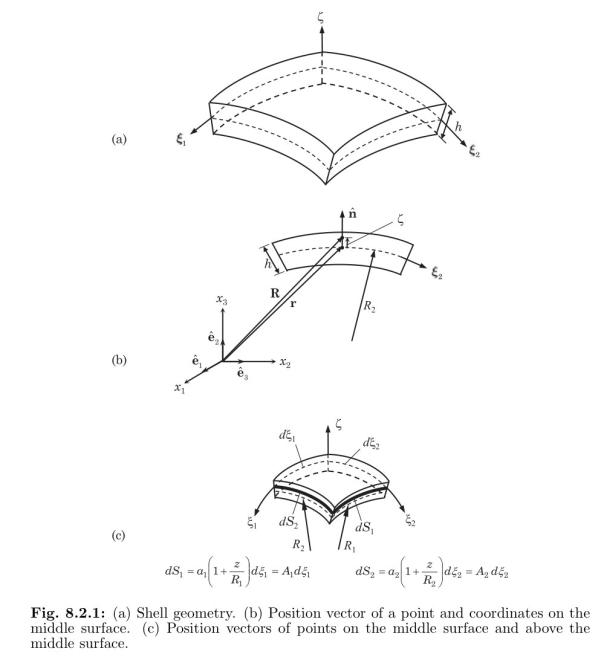
\includegraphics[width=0.65\linewidth]{Figure/fig48}  		
		\end{figure}
	\end{frame}


	\begin{frame}{Differential geometry}
		\begin{itemize}
			\item Take a curved shell element of uniform thickness. Here ($\xi_1,\xi_2,\zeta$) which denote the curvilinear coordinates such that $\xi_1, \xi_2$ curves are the lines of crvature of the middle surface ($\zeta = 0$). 
			\item The position vector of a point ($\xi_1,\xi_2,0$) is denote by $\ve{r}$ and any other arbitary point is denoted by $\ve{R}$
			\item A differential line element on the middle suface can be written as 
			\begin{equation}
			d\ve{r} = \frac{\partial \ve{r}}{\partial \xi_a}d\xi_a = \ve{g}_a d\xi_a , \quad \ve{g}_a = \frac{\partial \ve{r}}{\partial \xi_a} \quad (a =1,2)
			\end{equation}
			where the vectors $\ve{g}_1$ and $\ve{g}_2$ are tangent to the $\xi_1,\xi_2$ coordinates lines as shown.
			\item  The components of the metric tensor $g_{ab}$, (a,b=1,2) are 
			\begin{equation}
			\ve{g}_a.\ve{g}_b = g_{ab},  \qquad p_1 = \sqrt{g_{11}}, \qquad p_2 = \sqrt{g_{22}}, \qquad \ve{g_1.g_2} = p_1p_2cos \chi
			\end{equation}
			where $\chi$ denotes the angle between the coordinate curves. \footnote{Note that $\ve{\hat{n}},p_1,p_2$ are functions of $\xi_1,\xi_2$}
			\item The normal vector is found as
			\begin{equation}
			\ve{\hat{n}} = \frac{\ve{g_1 \times g_2}}{p_1p_2sin \chi}
			\end{equation}
		\end{itemize}	
	\end{frame}


	\begin{frame}{Differential geometry : continued}
		\begin{itemize}
			\item The square of the distance $dS$,say between points ($\xi_1,\xi_2,0$) and ($\xi_1 + d\xi_1,\xi_2+d\xi_2,0$) on th emiddle surface is given by
			\begin{equation}
			 (ds)^2 = d\ve{r}. d\ve{r} = g_{ab}d\xi_a d\xi_b = p_1^2(d\xi_1)^2 + p_2^2(d\xi_2)^2 + 2a_1a_2cos~\chi~d\xi_1 d\xi_2
			\end{equation}
			The RHS is called the first quadratic form of the surface which allows us to find infinitesimal lengths, angles and area. The terms $p_1^2,~p_2^2,~p_1p_2cos\chi$ are called the first fundamental quantities
			\item Let $\ve{r}= \ve{r}(s)$ be the equation of a curve $s$ on the surface. The unit vector tangent to the curve is
			\begin{equation}
				\ve{\hat{t}} =  \frac{d \ve{r}}{d   s} = \frac{\partial \ve{r}}{\partial \xi_a} \frac{\partial \xi_a}{\partial s} = \ve{g}_a \frac{\partial \xi_a}{\partial s}
			\end{equation}			
		\end{itemize}
	\end{frame}


	\begin{frame}{Governing E}
		Im not writing this because the conventions are too long. Please check the annotated book
	\end{frame}

\end{document}